\documentclass[letter,12pt]{article}
\usepackage[paperheight=27.94cm,paperwidth=21.59cm,bindingoffset=0in,left=3cm,right=2.0cm, top=3.5cm,bottom=2.5cm, headheight=200pt, headsep=1.0\baselineskip]{geometry}
\usepackage{graphicx,lastpage}
\usepackage{upgreek}
\usepackage{censor}
\usepackage[spanish,es-tabla]{babel}
\usepackage{pdfpages}
\usepackage{tabularx}
\usepackage{graphicx}
\usepackage{adjustbox}
\usepackage{xcolor}
\usepackage{colortbl}
\usepackage{rotating}
\usepackage{multirow}
\usepackage[utf8]{inputenc}
\usepackage{float}
\usepackage{hyperref}
\usepackage{seqsplit}

\renewcommand{\tablename}{Tabla}
\usepackage{fancyhdr}
\pagestyle{fancy}

\fancyhead[L]{}
%
\begin{document}
%
   \title{\Huge{Informe Laboratorio 4}}

   \author{\textbf{Sección 2} \\  \\Ignacio Cabrera \\ e-mail: ignacio.cabrera@mail.udp.cl}
          
   \date{Noviembre de 2024}

   \maketitle
   
   \tableofcontents
 
  \newpage
  

\section{Descripción de actividades}
Desarrollar un programa en Python utilizando la librería pycrypto para cifrar y descifrar mensajes con los algoritmos DES, AES-256 y 3DES, permitiendo la entrada de la key, vector de inicialización y el texto a cifrar desde la terminal. 

Instrucciones:

\begin{enumerate}
    \item Investigación
    \begin{itemize}
        \item Investigue y documente el tamaño en bytes de la clave y el vector de inicialización (IV) requeridos para los algoritmos DES, AES-256 y 3DES. Mencione las principales diferencias entre cada algoritmo, sea breve.
    \end{itemize}

    \item El programa debe solicitar al usuario los siguientes datos desde la terminal
    \begin{itemize}
        \item Key correspondiente a cada algoritmo.
        \item Vector de Inicialización (IV) para cada algoritmo.
        \item Texto a cifrar.
    \end{itemize}

    \item Validación y ajuste de la clave
    \begin{itemize}
        \item Si la clave ingresada es menor que el tamaño necesario para el algoritmo complete los bytes faltantes agregando bytes adicionales generados de manera aleatoria (utiliza get\_random\_bytes).
        \item Si la clave ingresada es mayor que el tamaño requerido, trunque la clave a la longitud necesaria.
        \item Imprima la clave final utilizada para cada algoritmo después de los ajustes.
    \end{itemize}

    \item Cifrado y Descifrado
    \begin{itemize}
        \item Implemente una función para cada algoritmo de cifrado y descifrado (DES, AES-256, y 3DES). Use el modo CBC para todos los algoritmos.
        \item Asegúrese de utilizar el IV proporcionado por el usuario para el proceso de cifrado y descifrado.
        \item Imprima tanto el texto cifrado como el texto descifrado.
    \end{itemize}

    \item Comparación con un servicio de cifrado online
    \begin{itemize}
        \item Selecciona uno de los tres algoritmos (DES, AES-256 o 3DES), ingrese el mismo texto, key y vector de inicialización en una página web de cifrado online.
        \item Compare los resultados de tu programa con los del servicio online. Valide si el resultado es el mismo y fundamente su respuesta.
    \end{itemize}

    \item Aplicabilidad en la vida real
    \begin{itemize}
        \item Describa un caso, situación o problema donde usaría cifrado simétrico. Defina que algoritmo de cifrado simétrico recomendaría justificando su respuesta.
        \item Suponga que la recomendación que usted entrego no fue bien percibida por su contraparte y le pide implementar hashes en vez de cifrado simétrico. Argumente cuál sería su respuesta frente a dicha solicitud. 
    \end{itemize}
\end{enumerate}



\section{Desarrollo de actividades según criterio de rúbrica}

\subsection{Investiga y documenta los tamaños de clave e IV}

A continuación se describirá cada algoritmo, los tamaños de clave e IV y sus diferencias entre cada uno. La información fue sacada del sitio web \url{https://www.pycryptodome.org/src/cipher/aes}.

\begin{itemize}
    \item DES: el tamaño de clave es de 8 bytes (64 bits), de los cuales solo 56 bits son efectivos para el cifrado, los 8 bits restantes son para control de paridad.
    
    Tamaño del IV: 8 bytes (64 bits).

    Actualmente se considera inseguro debido al tamaño reducido de su clave, lo que lo hace vulnerable a ataques de fuerza bruta. DES es rápido en hardware, pero su corta longitud de clave lo limita para aplicaciones modernas.

    \item AES-256: El tamaño de Clave es 32 bytes (256 bits).
    
    Tamaño del IV: 16 bytes (128 bits).

    AES-256 es uno de los algoritmos de cifrado más seguros y ampliamente utilizado en la actualidad, resistente a ataques de fuerza bruta. Es rápido y eficiente en hardware y software, y está optimizado para diversas plataformas.

    \item 3DES: El tamaño de clave es de 24 bytes (192 bits), que se dividen en tres claves de 8 bytes cada una.
    
    Tamaño del IV: 8 bytes (64 bits).

    Más seguro que DES al aplicar el cifrado tres veces, pero considerado menos seguro y eficiente que AES. Comparado con AES-256, es más lento debido al triple cifrado, lo que lo hace menos adecuado para aplicaciones modernas.
\end{itemize}


\subsection{Solicita datos de entrada desde la terminal}

Para poder iniciar esta actividad, se realiza el código en Python utilizando la librería pycrypto. Un fragmento del código se puede observar en la siguiente figura.

\begin{figure}[H]
    \centering
    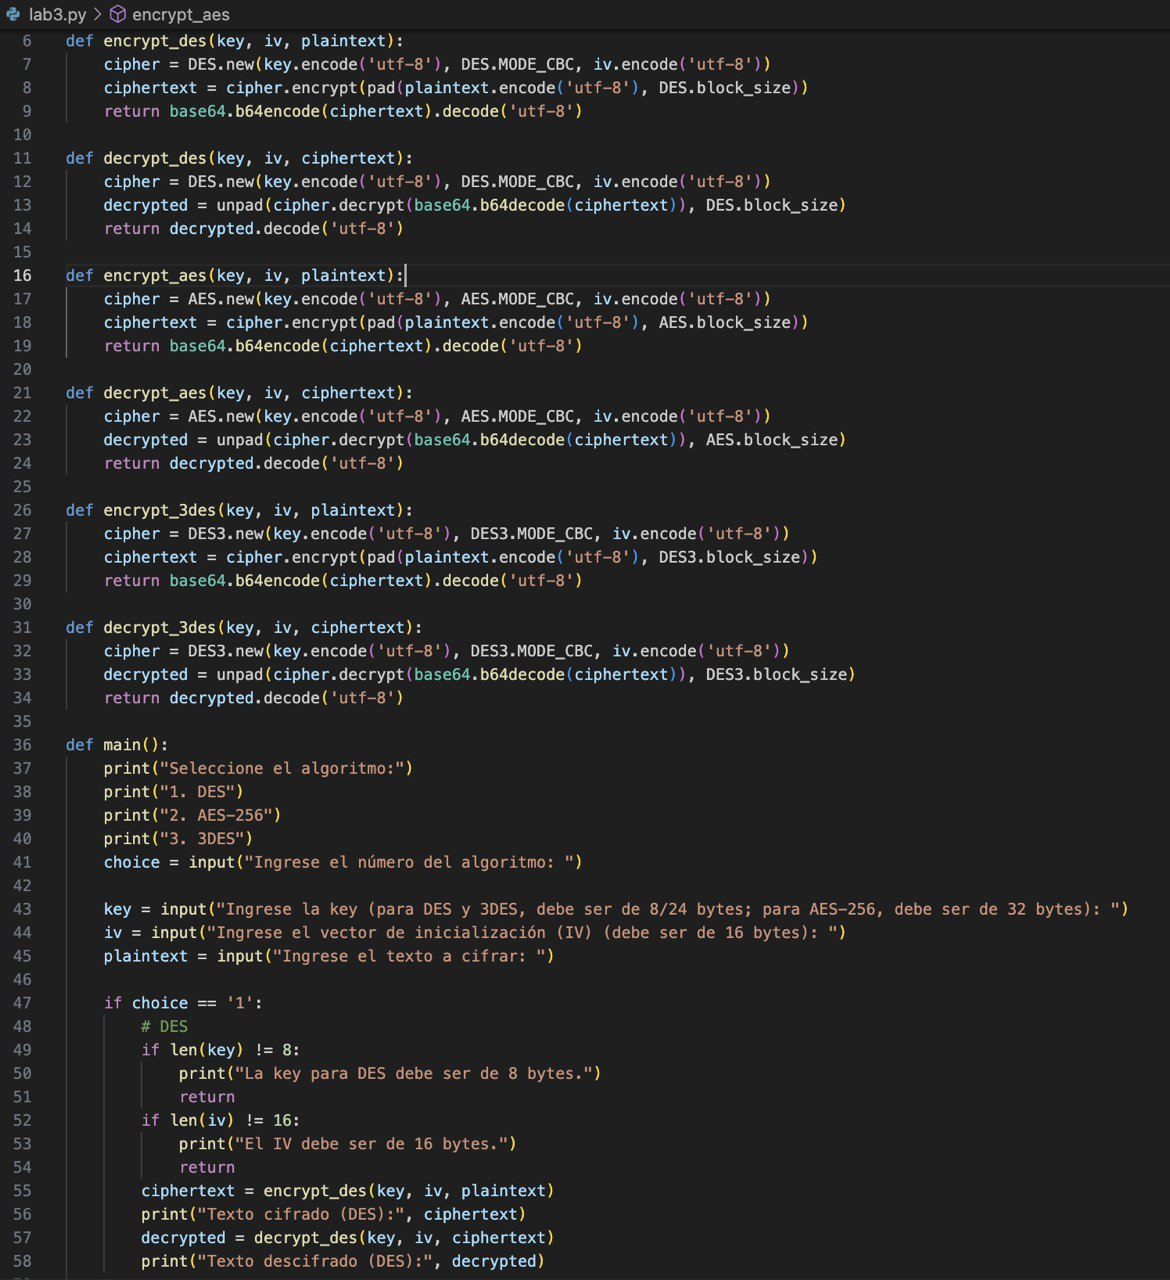
\includegraphics[width=0.9\linewidth]{imagenes/codigo 1.jpg}
    \caption{Fragmento de código Python utilizado}
    \label{fig:enter-label}
\end{figure}

Al ejecutar el código se solicita los datos de entradas correspondientes, como se puede observar en la siguiente figura.

\begin{figure}[H]
    \centering
    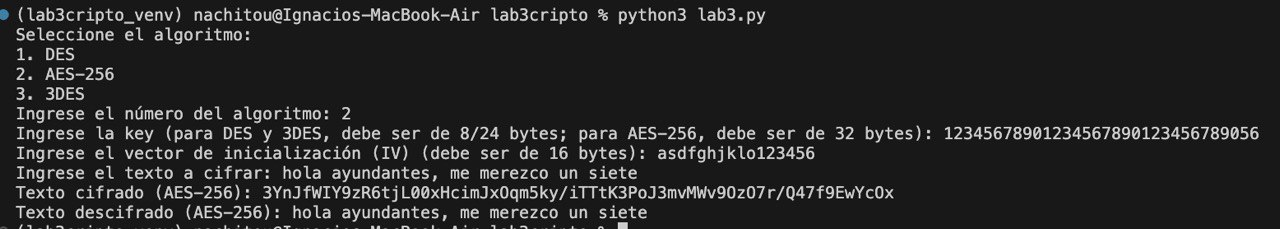
\includegraphics[width=0.9\linewidth]{imagenes/salida 1.jpg}
    \caption{Salida y solicitación de datos}
    \label{fig:enter-label}
\end{figure}

Como se puede observar en la figura anterior, se le pide al usuario que seleccione el algoritmo que quiere utilizar, en este caso como ejemplo es el algoritmo AES-256. También solicita la key correspondiente, el vector de inicialización y el texto a cifrar, que en este caso fue ''hola ayundantes, me merezco un siete", donde la salida del texto cifrado, en este caso AES-256 fue de ''3YnJfWIY9zR6tjL00xHcimJxOqm5ky/iTTtK3PoJ3mvMWv9OzO7r/Q47f9EwYcOx"  

\subsection{Valida y ajusta la clave según el algoritmo}

Para realizar la actividad, se reemplaza el código anterior con las nuevas funcionalidades, para así cumplir con lo solicitado. El fragmento del código se puede observar en la siguiente figura.

\begin{figure}[H]
    \centering
    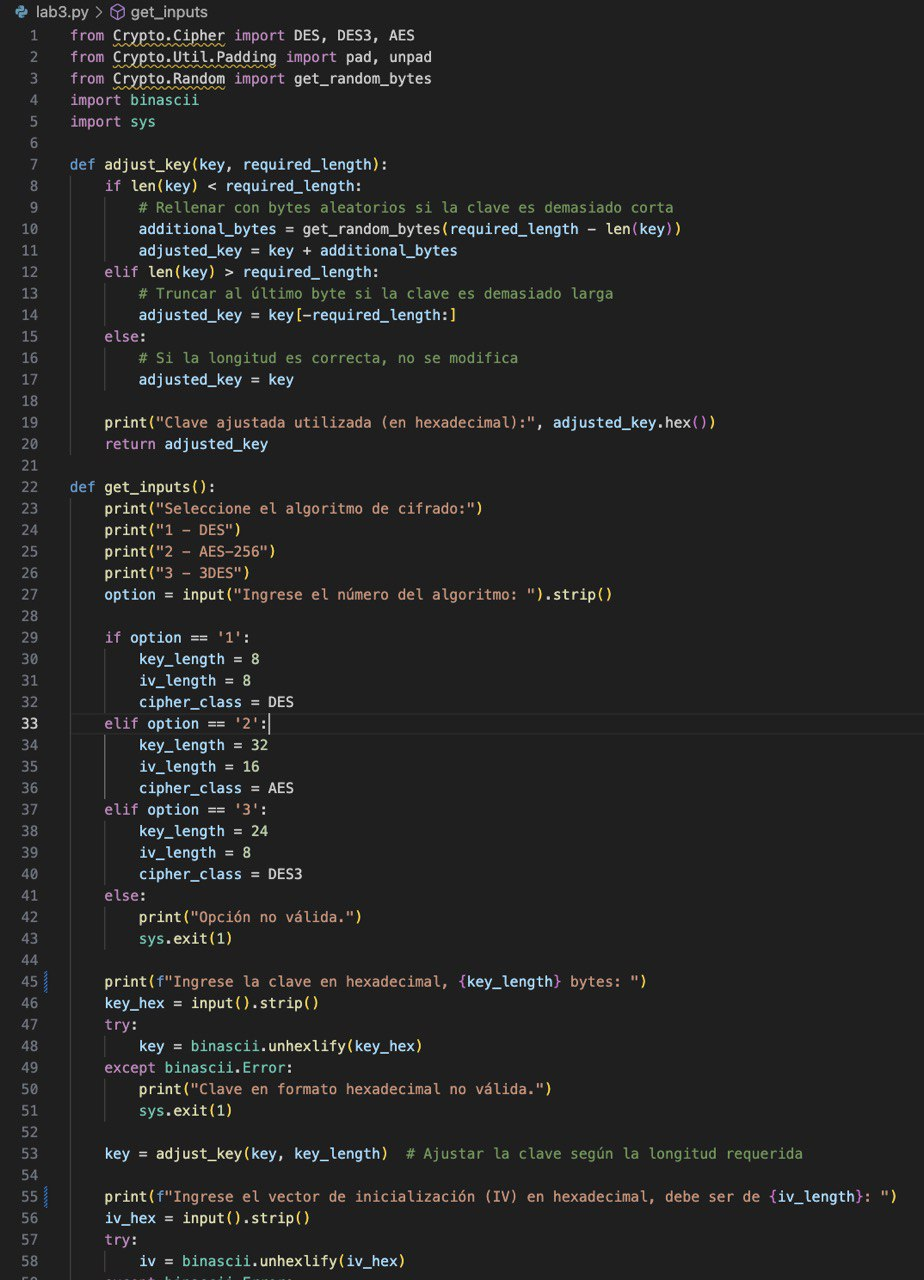
\includegraphics[width=0.8\linewidth]{imagenes/codigo 2.jpg}
    \caption{Fragmento de código Python}
    \label{fig:enter-label}
\end{figure}

Al ejecutar el código anterior, la salida es la mismo que la que la figura 2, pero se truncará si la clave ingresada es mayor que la longitud necesaria para el algoritmo. Y si la clave ingresada es menor que el tamaño necesario, se agregarán los bytes adicionales de manera aleatoria. A continuación se observará cuando las claves son truncadas.

\subsubsection{Truncación}


\begin{figure}[H]
    \centering
    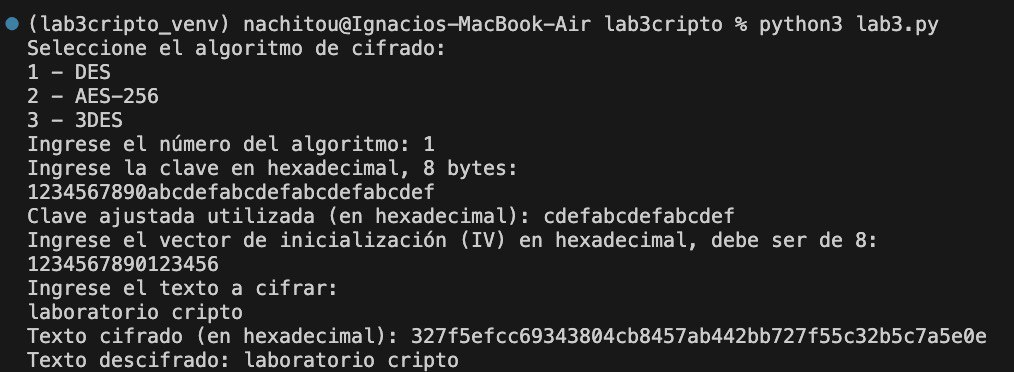
\includegraphics[width=0.8\linewidth]{imagenes/truncar.jpg}
    \caption{Clave truncada a 8 bytes. Algoritmo DES}
    \label{fig:enter-label}
\end{figure}

En la figura anterior se puede observar que se seleccionó el algoritmo de DES, donde la clave colocada por el usuario fue de \seqsplit{''1234567890abcdefabcdefabcdefabcdef"}. Esta clave es mayor que el tamaño requerido, por lo tanto se truncó de izquierda a derecha, teniendo el resultado de '' cdefabcdefabcdef". A continuación se podran observar el resultado de los otros algoritmos.

\begin{figure}[H]
    \centering
    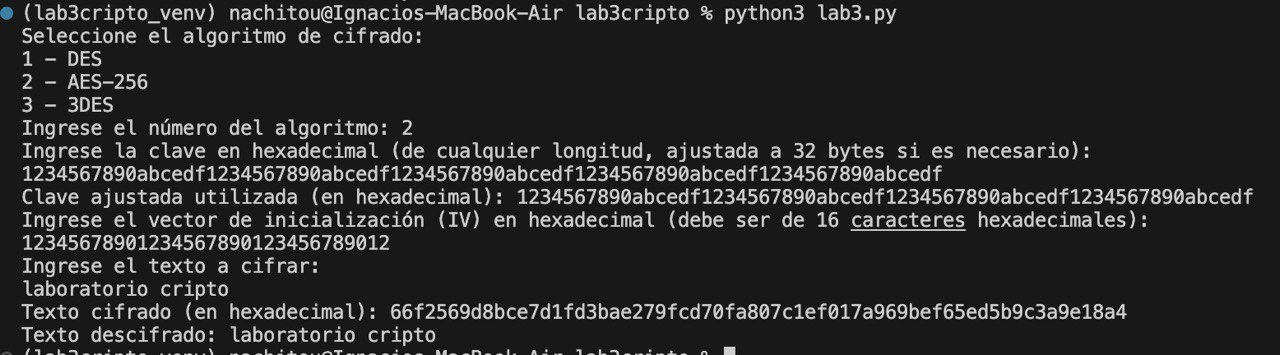
\includegraphics[width=1.0\linewidth]{imagenes/truncar aes.jpg}
    \caption{Clave truncada. Algoritmo AES-256}
    \label{fig:enter-label}
\end{figure}

En el algoritmo AES-256, la clave ejecutada por el usuario fue de \seqsplit{''1234567890abcedf1234567890abcedf1234567890abcedf1234567890abcedf1234567890abcedf"}, y la clave ajustada al tamaño del algoritmo AES-256, fue de \seqsplit{''1234567890abcedf1234567890abcedf1234567890abcedf1234567890abcedf"}.

\begin{figure}[H]
    \centering
    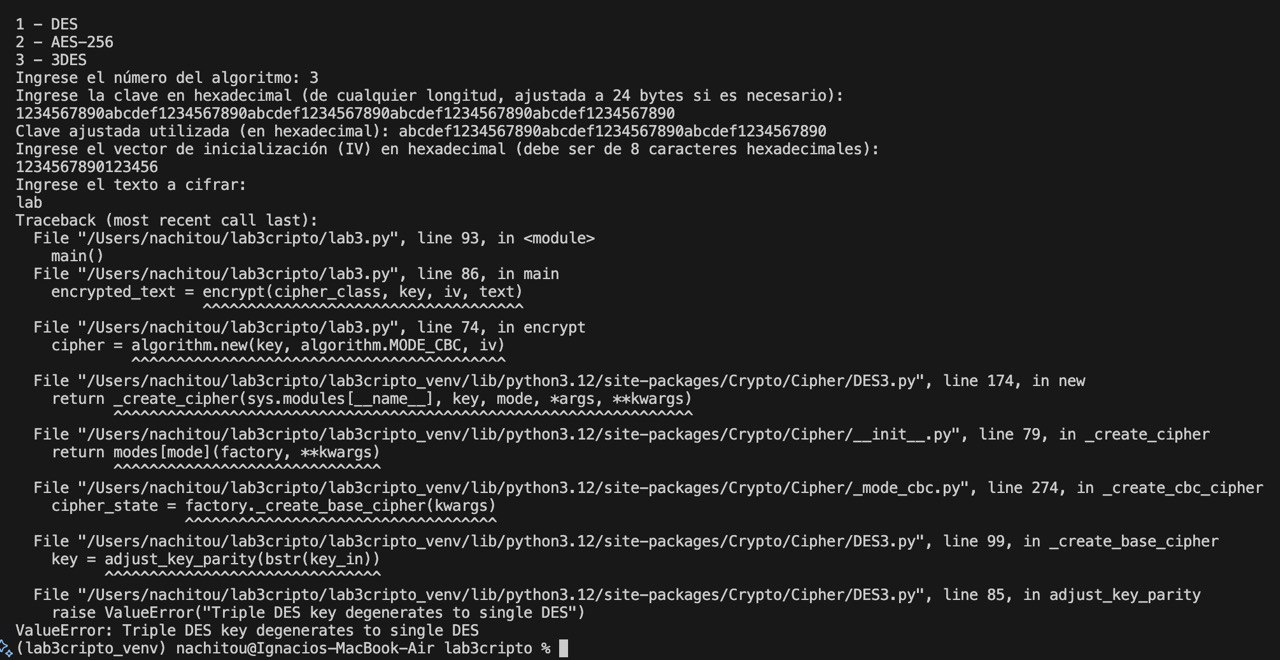
\includegraphics[width=0.9\linewidth]{imagenes/DES fallo.jpg}
    \caption{Error en algormitmo 3DES}
    \label{fig:enter-label}
\end{figure}

De primera instancia para el Algoritmo 3DES, compilaba el error que sale en la figura anterior, pero es porque para el algoritmo 3DES, las subclaves deben ser únicas, ya que si se identifica un patrón, el cifrado 3DES se convertirá en un DES simple, anulando la sefuridad adicional. En la siguiente figura se observa el resultado con truncación.


\begin{figure}[H]
    \centering
    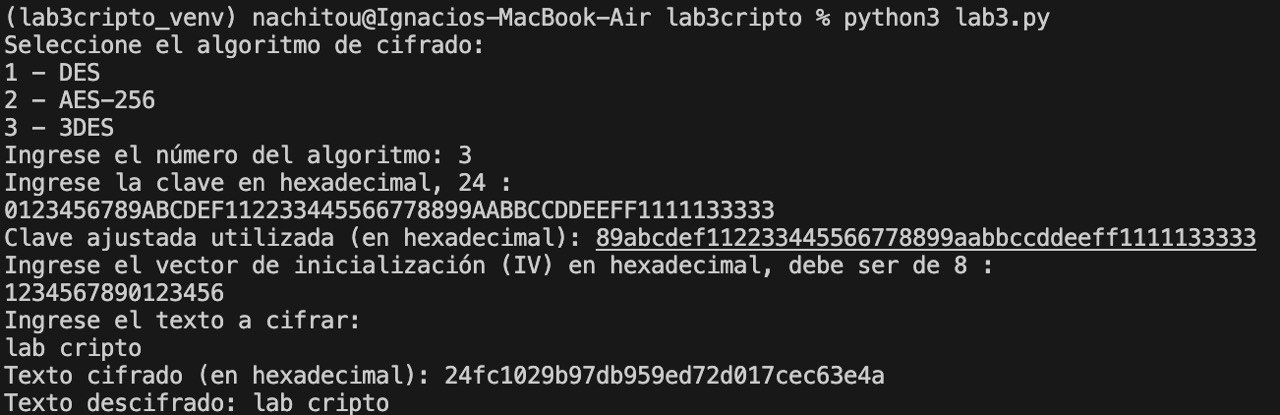
\includegraphics[width=0.8\linewidth]{imagenes/truncado 3des.jpg}
    \caption{Clave truncada. Algoritmo 3DES}
    \label{fig:enter-label}
\end{figure}

La clave ejecutada por el usuario fue \seqsplit{''0123456789ABCDEF112233445566778899AABBCCDDEEFF1111133333"}, donde la clave ajustada al tamaño del algoritmo 3DES fue \seqsplit{''89abcdef112233445566778899aabbccddeeff1111133333"}. Dando un correcto resultado.


\subsubsection{Agregar Bytes}

A continuación se podrá observar, cuando se agregan los bytes faltantes para cada uno de los 3 algoritmos.

\begin{figure}[H]
    \centering
    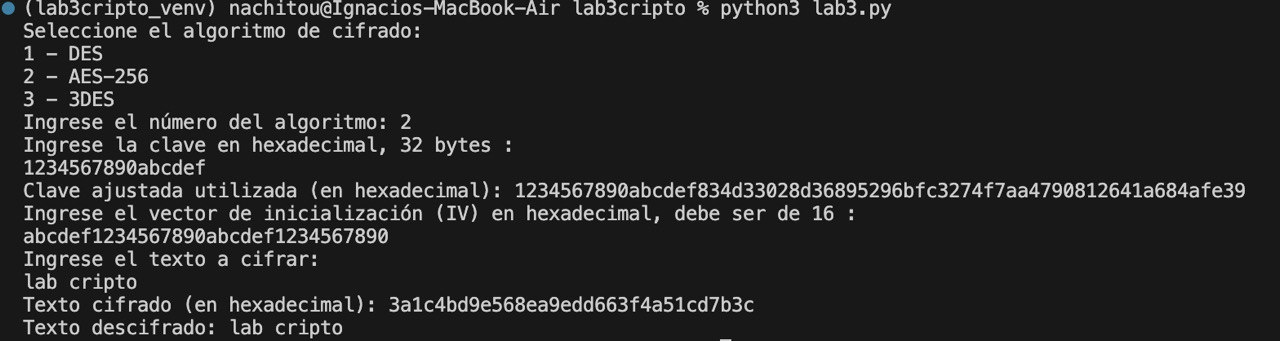
\includegraphics[width=0.8\linewidth]{imagenes/aes generar.jpg}
    \caption{Agregar bytes faltantes. Algoritmo AES-256}
    \label{fig:enter-label}
\end{figure}
La key entregada por el usuario fue de ''1234567890abcdef", donde se ajustó a \seqsplit{''1234567890abcdef834d33028d36895296bfc3274f7aa4790812641a684afe39"}.

\begin{figure}[H]
    \centering
    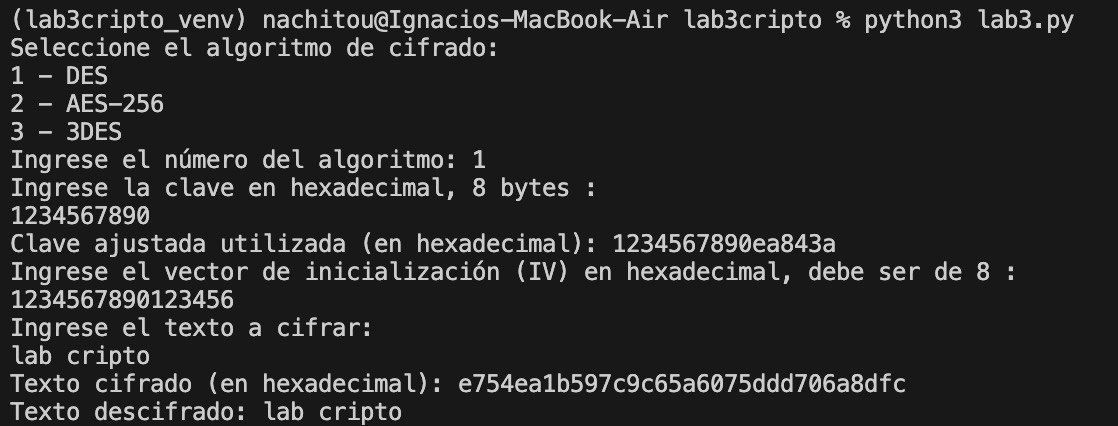
\includegraphics[width=0.8\linewidth]{imagenes/des generar.jpg}
    \caption{Agregar bytes faltantes. Algoritmo Des}
    \label{fig:enter-label}
\end{figure}

La key por el usuario fue de ''1234567890", donde se ajustó a ''1234567890ea843a".

\begin{figure}[H]
    \centering
    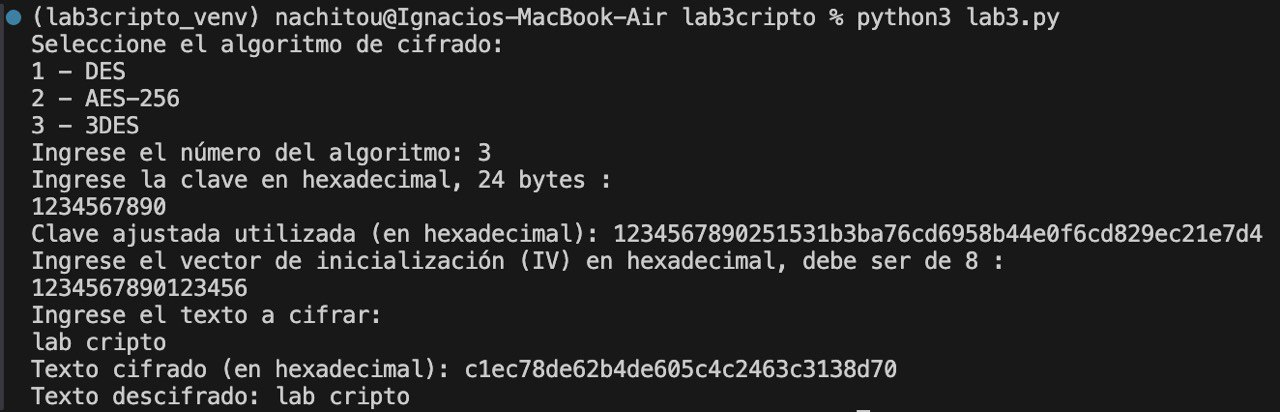
\includegraphics[width=0.8\linewidth]{imagenes/3des generar.jpg}
    \caption{Agregar bytes faltantes. Algoritmo 3DES}
    \label{fig:enter-label}
\end{figure}

La key entregada por el usuario fue de ''1234567890", donde se ajustó a \seqsplit{''1234567890251531b3ba76cd6958b44e0f6cd829ec21e7d4"}.


\subsection{Implementa el cifrado y descifrado en modo CBC}
Para poder cumplir con el cifrado CBC y su descifrado, se tuvo que crear las funciones correspodientes para este cifrado, lo que se observará en la siguiente figura.

\begin{figure}[H]
    \centering
    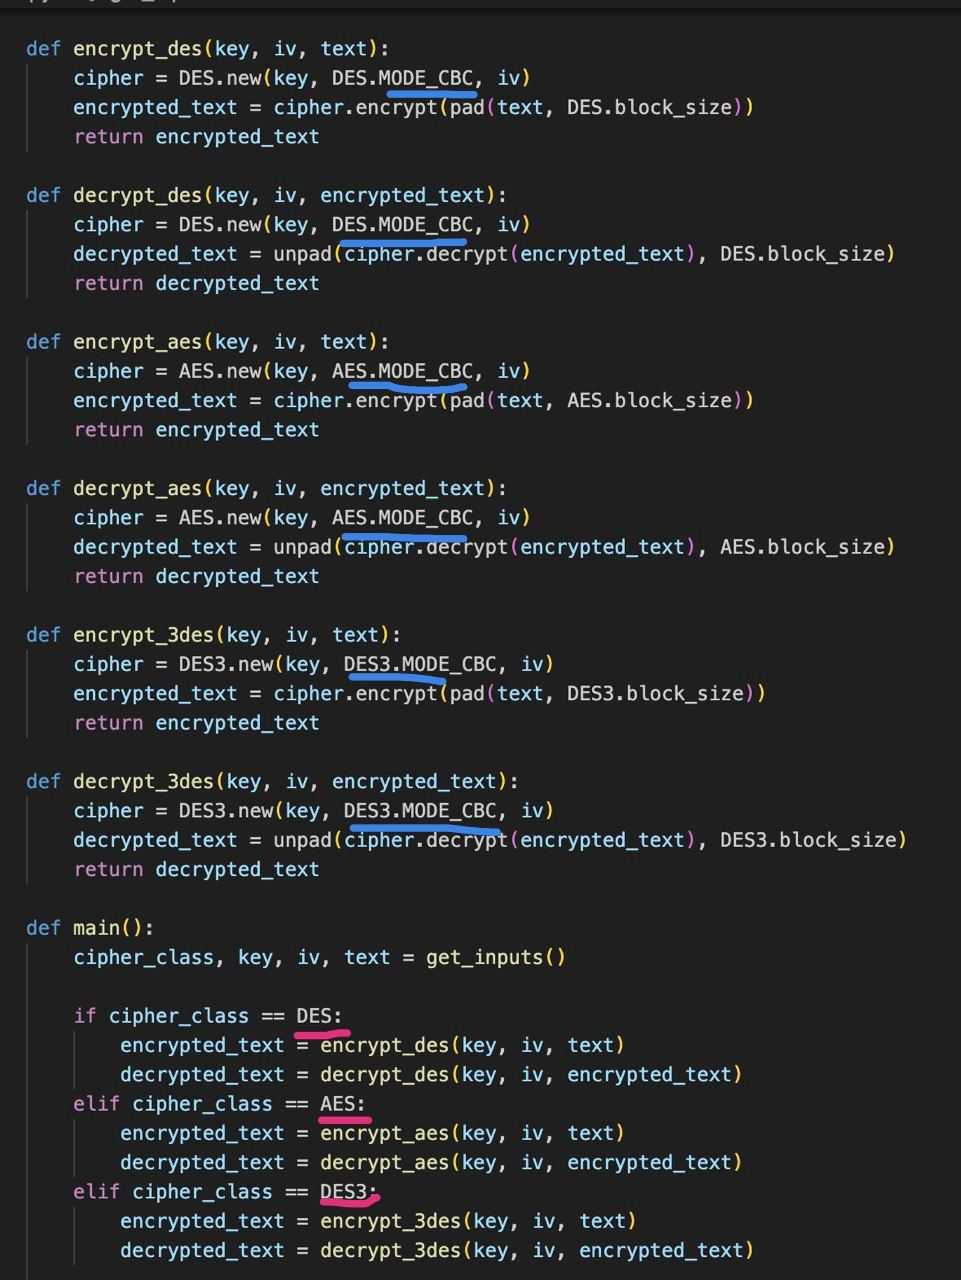
\includegraphics[width=0.8\linewidth]{imagenes/codigo cbc.jpg}
    \caption{Función para cifrado CBC.}
    \label{fig:enter-label}
\end{figure}

Ya aplicadas las funciones se procede a ejecutar el código. Para la correcta implementación se tiene que seleccionar un vector de Inicialización diferente a los ejecutados anteriormente, para que dé un resultado diferente. Esto se debe a que CBC no introduce aleatoriedad por sí mismo, en lugar de eso, depende de que cada bloque de texto cifrado esté ligado al bloque anterior y del IV. A continuación se podra observar para los tres algoritmos seleccionados.


\begin{figure}[H]
    \centering
    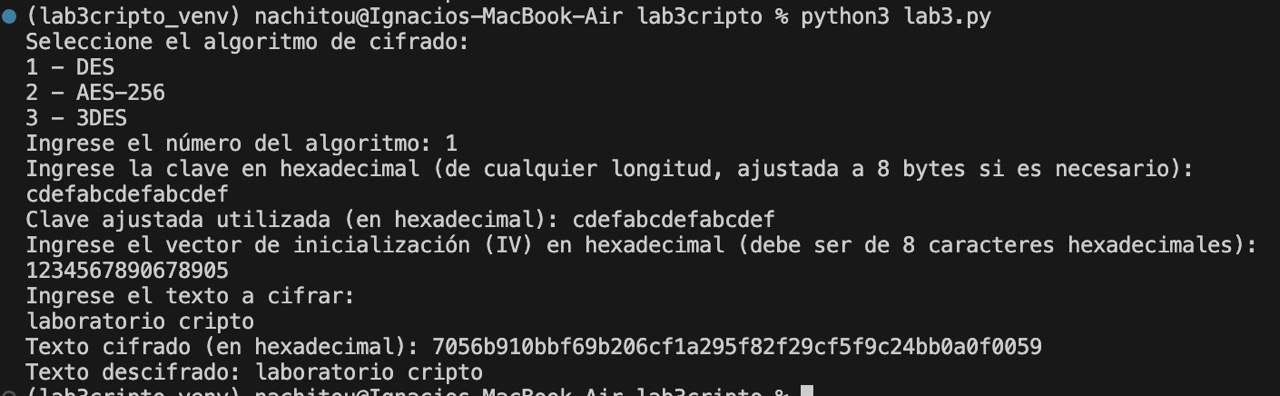
\includegraphics[width=0.8\linewidth]{imagenes/cbc des.jpg}
    \caption{Algoritmo DES con CBC}
    \label{fig:enter-label}
\end{figure}


\begin{figure}[H]
    \centering
    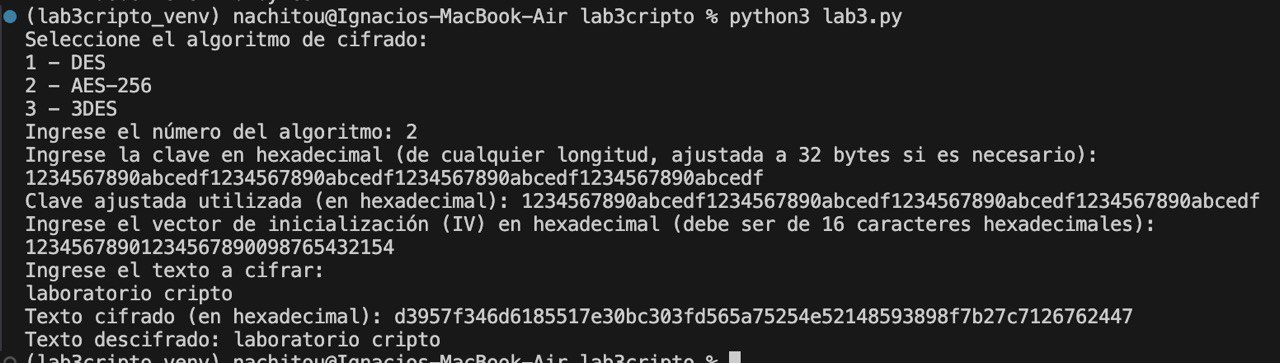
\includegraphics[width=0.8\linewidth]{imagenes/cbc aes.jpg}
    \caption{Algoritmo AES-256 con CBC}
    \label{fig:enter-label}
\end{figure}

\begin{figure}[H]
    \centering
    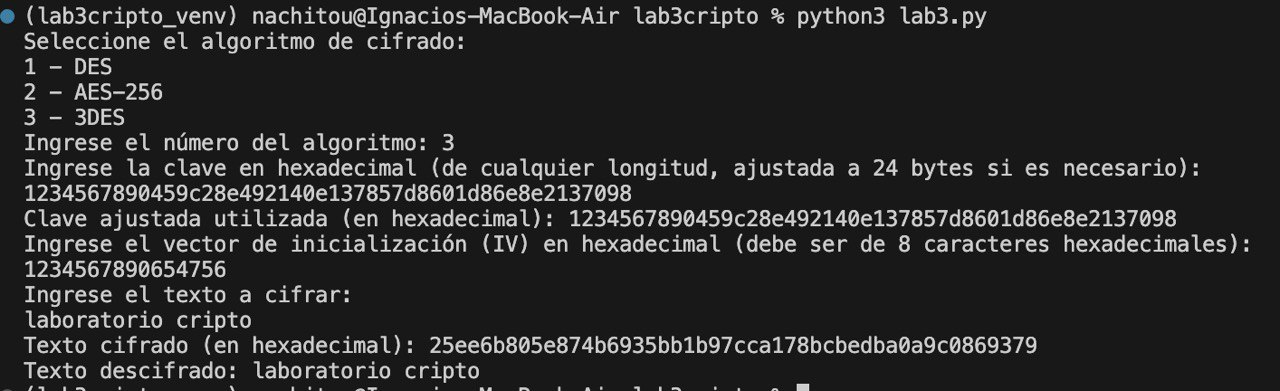
\includegraphics[width=0.8\linewidth]{imagenes/cbc 3des.jpg}
    \caption{Algoritmo 3DES con CBC}
    \label{fig:enter-label}
\end{figure}

Como el texto cifrado cambió drasticamente cuando se cambió solamente el IV, el modo CBC funcionó correctamente en la implementación.





\subsection{Compara los resultados con un servicio de cifrado online}

Para poder completar esta sección, se seleccionó el algoritmo AES-256, donde se utilizo la página \url{https://gchq.github.io/CyberChef/}. Como la llave se puso el texto \seqsplit{''1234567890abcedf1234567890abcedf1234567890abcedf1234567890abcedf"} y como vector de inicialización ''12345678901234567890123456789012", estos parametros entregados son los mismos que los de la figura 5. Al poner las credenciales en el servicio de cifrado online, se obtuvo el siguiente resultado.


\begin{figure}[H]
    \centering
    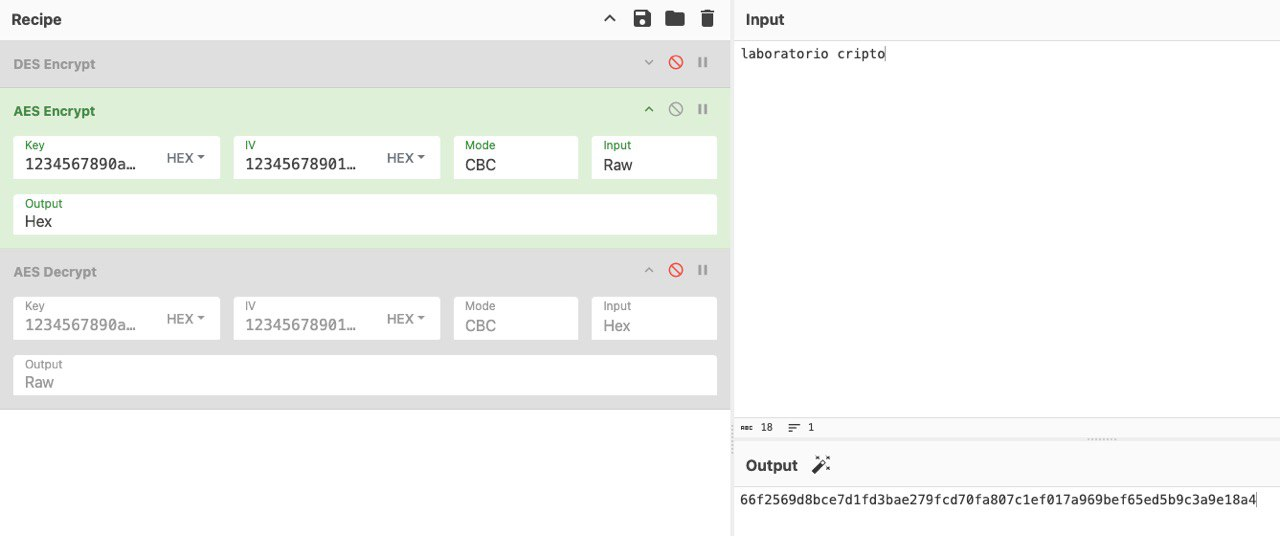
\includegraphics[width=1.0\linewidth]{imagenes/cifrar online aes.jpg}
    \caption{Cifrado online}
    \label{fig:enter-label}
\end{figure}

\begin{figure}[H]
    \centering
    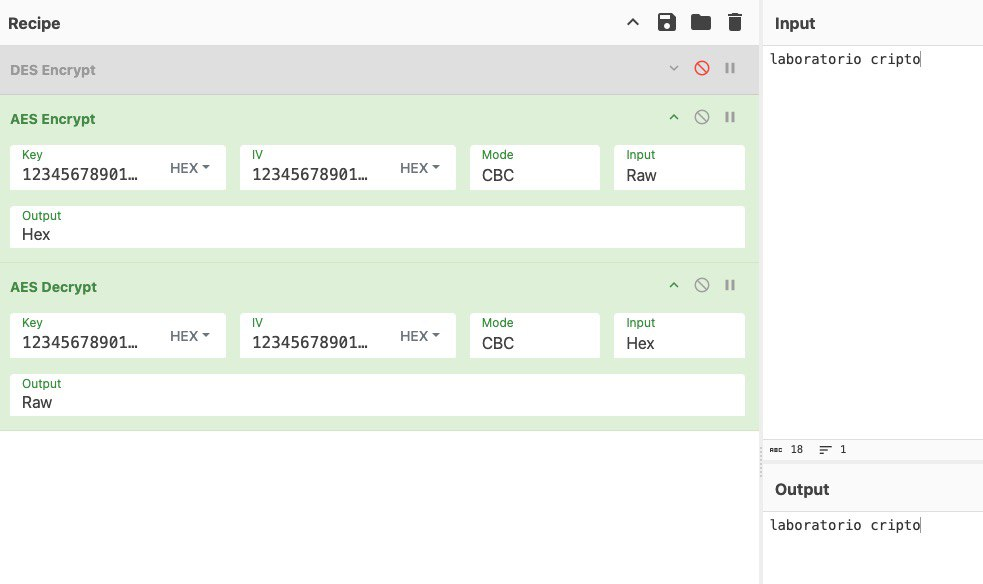
\includegraphics[width=1.0\linewidth]{imagenes/descript web aes.jpg}
    \caption{Texto descifrado}
    \label{fig:enter-label}
\end{figure}

Como se puede observar, entrega el mismo output que el de la figura 5 que es \seqsplit{"66f2569d8bce7d1fd3bae279fcd70fa807c1ef017a969bef65ed5b9c3a9e18a4"}. Además, el descifrado coincide con el texto puesto por el usuario.

El resultado es el mismo porque tanto el código como el cifrado online utilizaron la misma configuración de clave, IV y texto, y el modo CBC es determinista bajo estas condiciones. Este comportamiento es una propiedad fundamental del cifrado simétrico y permite que el cifrado sea replicable y verificable en diferentes entornos. Cabe recalcar que AES-256 es un estándar que sigue una especificación rigurosa, cualquier implementación de AES-256 en CBC debería producir el mismo resultado con los mismos parámetros. Además, no hay aleatoriedad adicional en la operación cuando se proporciona un IV específico, la aleatoriedad se introduce solo al cambiar el IV, la clave o el texto.


\subsection{Describe la aplicabilidad del cifrado simétrico en la vida real}

\section*{Conclusiones y comentarios}

% Please add the following required packages to your document preamble:
%\begin{table}[htbp]

\end{document}
